\documentclass[a4paper,14pt]{article}
\usepackage{float}
\usepackage{extsizes}
\usepackage{amsmath}
\usepackage{amssymb}
\everymath{\displaystyle}
\usepackage{geometry}
\usepackage{fancyhdr}
\usepackage{multicol}
\usepackage{graphicx}
\usepackage[brazil]{babel}
\usepackage[shortlabels]{enumitem}
\usepackage{cancel}
\usepackage{textcomp}
\usepackage{array} % Para melhor formatação de tabelas
\usepackage{longtable}
\usepackage{booktabs}  % Para linhas horizontais mais bonitas
\usepackage{float}   % Para usar o modificador [H]
\usepackage{caption} % Para usar legendas em tabelas

\columnsep=2cm
\hoffset=0cm
\textwidth=8cm
\setlength{\columnseprule}{.1pt}
\setlength{\columnsep}{2cm}
\renewcommand{\headrulewidth}{0pt}
\geometry{top=1in, bottom=1in, left=0.7in, right=0.5in}

\pagestyle{fancy}
\fancyhf{}
\fancyfoot[C]{\thepage}

\begin{document}
	
	\noindent\textbf{6FMA93 - Matemática} 
	
	\begin{center}Expressões com letras (Versão estudante)
	\end{center}
	
	\noindent\textbf{Nome:} \underline{\hspace{10cm}}
	\noindent\textbf{Data:} \underline{\hspace{4cm}}
	
	%\section*{Questões de Matemática}
	~ \\ ~
	\begin{multicols}{2}
	\noindent Em uma expressão aritmética em que um número foi substituído por um símbolo (como um quadrado ou uma letra), é possível descobrir o valor do número representado pelo símbolo, desde que se conheça o valor da expressão. \\
	Por exemplo: \\
	\begin{equation*}
		\square + 4 = 9
	\end{equation*}
	A ideia é simples: se o número procurado, acrescido de 4 unidades, vale 9, então, se retirarmos 4 unidades de 9, vamos encontrar o número procurado.
	\begin{equation*}
		\square = 9 - 4, \text{ou seja,~} \square = 5
	\end{equation*}
	Observe que resolvemos o problema usando o fato de que a subtração é a operação inversa da adição. \\
	Na expressão \\
	\begin{equation*}
		4 \cdot \square = 20,
	\end{equation*}
	queremos descobrir qual número devemos escrever no quadradinho para que a igualdade se torne verdadeira. \\
	Mais uma vez, a ideia é simples: se o número procurado, ao ser multiplicado por 4, vale 20, então, se dividirmos 20 por 4, vamos encontrar o número procurado.
	\begin{equation*}
		\square = \frac{20}{4}, \text{ou seja,~} \square = 5
	\end{equation*}
	Observe que resolvemos o problema usando o fato de que a divisão é a operação inversa da multiplicação.
	\end{multicols}
\noindent\textsubscript{~-----------------------------------------------------------------------------------------------------------------------------------------------------}
	\begin{multicols}{2}
    	\begin{enumerate}
    		\item Em cada caso a seguir, diga qual número deve ser escrito no quadradinho para tornar verdadeira a igualdade.
    		\begin{enumerate}[a)]
    			\item $\square + 7 = 32$ \\\\\\
    			\item $36 + \square = 84$ \\\\\\
    			\item $97 = \square + 52$ \\\\\\
    			\item $\square - 8 = 46$ \\\\\\
    			\item $63 - \square = 39$ \\
    			\item $97 = \square - 36$ \\\\\\
    		\end{enumerate}
    		\item Qual número está representado pela letra em cada uma das igualdades a seguir?
    		\begin{enumerate}[a)]
    			\item $x + 27 = 176$ \\\\\\
    			\item $y + 8 = 8 + 15$ \\\\\\
    			\item $74 = 78 + z$ \\\\\\
    			\item $45 - w = 43$ \\\\\\
    			\item $96 = p - 22$ \\\\\\
    			\item $q - 188 = 1888$ \\\\\\
    		\end{enumerate}
    		\item Em cada caso a seguir, diga qual número deve ser escrito no quadradinho para tornar verdadeira a igualdade.
    		\begin{enumerate}[a)]
    			\item $\square \cdot 9 = 45$ \\
    			\item $9 \cdot \square = 72$ \\\\\\
    			\item $42 = \square \cdot 7$ \\\\\\
    			\item $\square \cdot 8 = 32$ \\\\\\
    			\item $6 \cdot \square = 84$ \\\\\\
    			\item $145 = \square \cdot 5$ \\\\\\
    			\item $\square : 4 = 20$ \\\\\\
    			\item $\square : 5 = 17$ \\\\\\
    			\item $\frac{\square}{9} = 14$ \\\\\\ 
    		\end{enumerate}
    		\item Qual número está representado pela letra, em cada uma das igualdades a seguir?
    		\begin{enumerate}[a)]
    			\item $x \cdot 4 = 64$ \\
    			\item $7 \cdot y = 210$ \\\\\\
    			\item $10z = 80$ \\\\\\
    			\item $8t = 88$ \\\\\\
    			\item $129 = 43x$ \\\\\\
    			\item $196 = 14y$ \\\\\\
    			\item $z : 3 = 9$ \\\\\\
    			\item $x : 4 = 8$ \\\\\\
    			\item $\frac{y}{5} = 17$ \\\\\\
    		\end{enumerate}
    		\item Sabe-se que $u = 24$. Diga qual é o valor de:
    		\begin{enumerate}[a)]
    			\item $4 + u$ \\\\\\
    			\item $4u$ \\\\\\
    			\item $4 - u$ \\\\\\
    			\item $\frac{u}{4}$ \\\\\\
    		\end{enumerate}
    		\textbf{Desafio olímpico} \\\\
    		Ana e sua prima Beatriz fazem aniversário no mês de maio. No dia 23 de agosto de 2018, Ana somou sua idade com a idade de Beatriz e também com o seu ano de nascimento e o ano de nascimento de sua prima. Ao final, ela dividiu o resultado por 4. Qual o valor que Ana encontrou?
    		\begin{enumerate}[a)]
    			\item 862
    			\item 948
    			\item 1009
    			\item 2048
    			\item 3610 \newpage
    		\end{enumerate}
    		\item Em cada item a seguir, determine o número que deve ser escrito no quadradinho para tornar a igualdade verdadeira.
    		\begin{enumerate}[a)]
    			\item $\square - 13 = 28$
    			\item $24 + \square = 57$
    			\item $146 = \square + 87$
    			\item $27 - \square = 13$
    			\item $54 - \square = 47$
    			\item $76 = 143 - \square$
    		\end{enumerate}
    		\item Em cada uma das igualdades a seguir, determine o número que está representado pela letra.
    		\begin{enumerate}[a)]
    			\item $x + 11 = 32$
    			\item $9 + y = 52$
    			\item $249 + z = 487$
    			\item $389 = 604 - r$
    			\item $28 + x = 44$
    			\item $104 = y + 142$
    			\item $55 - z = 36$
    			\item $89 = r - 36$
    		\end{enumerate}
    		\item \begin{enumerate}[a)]
    			\item Se $x = 9$, quanto vale $x + 12$?
    			\item Se $y = 21$, quanto vale $y - 7$?
    			\item Se $a = 4$, quanto vale $8 - (a - 2)$? \\\\\\\\\\\\
    		\end{enumerate}
    		\item Daniel pretendia comprar uma bicicleta de 720 reais. Após juntar uma certa quantia, ele notou que faltaram 80 reais para comprá-la. Qual é o valor que Daniel juntou? \\\\\\\\\\\\\\\\\\
    		\item Júlio mora com seus dois irmãos e eles decidiram comprar uma poltrona de 230 reais. Júlio contribuirá com 75 reais e seu irmão mais velho com 105 reais. Qual é o valor que o irmão mais novo precisará contribuir para que eles comprem a poltrona? \\\\\\\\\\\\\\\\\\\\\\\\\\\\\\\\\\
    		\item No diagrama a seguir, a soma dos números em cada linha (horizontal, vertical ou diagonal) é sempre a mesma. Quanto vale $(x - y) - w + z$?
    		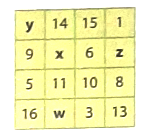
\includegraphics[width=1\linewidth]{imagens_6FMA93/imagem1} \\\\\\\\\\\\\\\\\\
    		\item No diagrama a seguir, a soma de dois quadrados consecutivos resulta no quadrado acima deles. Por exemplo, 2 + 3 = 5: \\
    		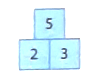
\includegraphics[width=0.5\linewidth]{imagens_6FMA93/imagem2} \\
    		Quanto valem $x, y $ e $z$? \\
    		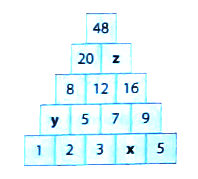
\includegraphics[width=1\linewidth]{imagens_6FMA93/imagem3} \\
    		\item Para $y = 19$, determine o valor da expressão:
    		\begin{equation*}
    			(y + 15) \cdot (y - 17) + 19y - \frac{19}{y}
    		\end{equation*}
    		\item Para $x = 9$, determine o valor da expressão:
    		\begin{equation*}
    			(x + 1) \cdot (18 - x) + \frac{13}{x} - \frac{63}{x} + \frac{x - 5}{x + 3}
    		\end{equation*}
    		\item Em cada item a seguir, determine o número que deve ser escrito no quadradinho para tornar a igualdade verdadeira.
    		\begin{enumerate}[a)]
    			\item $\square \cdot 5 = 35$
    			\item $\square \cdot 8 = 72$
    			\item $28 = \square \cdot 7$
    			\item $5 \cdot \square = 45$ 
    			\item $9 \cdot \square = 126$
    			\item $108 = \square \cdot 6$
    			\item $\square : 4 = 8$
    			\item $\square : 9 = 6$
    			\item $\frac{\square}{7} = 13$ 
    		\end{enumerate}
    		\item Qual número está representado pela letra em cada uma das igualdades a seguir?
    		\begin{enumerate}[a)]
    			\item $x \cdot 6 = 78$
    			\item $4 \cdot y = 84$
    			\item $10z = 50$ 
    			\item $3r = 999$
    			\item $144 = 48x$
    			\item $256 = 16y$
    			\item $z:7 = 8$
    			\item $r:6 = 11$
    			\item $\frac{x}{9} = 13$ \\\\\\\\\\\\\\\\\\\\\\\\\\\\\\\\\\\\\\\\\\\\\\\\\\\\
    		\end{enumerate}
    		\item Seja $a = 6 + 3 \cdot (5 - 1)$ e $b = (21 - 17) \cdot 2 - 6$. Dizer qual é o valor de:
    		\begin{enumerate}[a)]
    			\item $a + b$
    			\item $b + a$
    			\item $a - b$
    			\item $b - a$
    			\item $a \cdot b$
    			\item $b \cdot a$
    			\item $a : b$
    			\item $\frac{a}{b}$
    			\item $\frac{b}{a}$
    		\end{enumerate}
    	\end{enumerate}
    $~$ \\ $~$ \\ $~$ \\ $~$ \\ $~$ \\ $~$ \\ $~$ \\ $~$ \\ $~$ \\ $~$ \\ $~$ \\ $~$ \\ $~$ \\ $~$ \\ $~$ \\ $~$ \\ $~$ \\ $~$ \\ $~$ \\ $~$ \\ $~$ \\ $~$ \\ $~$ \\ $~$ \\ $~$
	\end{multicols}
\end{document}